\chapter{社交网络中传播效率最大化}
\label{3chap:main}
\textbf{影响力最大化}(\textit{Influence Maximization})在许多的社交网络应用中扮演着举足轻重的角色,例如市场营销、商业活动以及竞选活动等等。研究信息传播模型以及机理的一个典型目的便是市场营销。在现实社会中,人或者事物都是通过某种关系来连接,形成了一个巨大的网络。因此,信息传播可以选择一小部分节点激活做为种子节点集合,然后通过信息的传递,在整个网络中产生一个大范围的影响。从技术方面来说,影响力最大化问题是在给定网络和传播模型的条件下,研究如何选择种子节点集合使得传播的影响范围最大化。影响力最大化问题由于其的问题真实、应用性广的特点,吸引了许许多多的研究,包括信息传播模型的研究和计算影响力最大化的方法。但是,仍然有着一些需求在实际应用中得不到满足。

在信息传播过程中,一个被激活的节点将会尝试在下一个时刻激活它的邻居节点。所以,除去种子节点外,每一个被激活的节点在被激活之前都会有一个时间延迟,我们称之为\textbf{传播时延}(\textit{propagation time delay})。如果一个节点在信息传播结束时,仍然未被激活,则该节点的传播时延可以看作无穷大。在传统的影响力最大化问题中,传播时延没有被考虑在内,而研究整个网络的传播时延是非常有意义的,它可以度量选择的种子节点集合的传播效率。出于这种需求,本章提出了一个新的问题,传播效率最大化问题。该问题将传播时延考虑在内,在给定网络和传播模型的条件下,研究如何选择种子节点集合使得传播效率最大化。传播效率最大化问题与影响力最大化问题虽然相似,但是两个问题的侧重点不尽相同。传统的影响力最大化问题研究的是如何使得传播的范围最广,不考虑节点的传播时延。而本章提出的传播效率最大化问题将传播时延考虑在内,研究如何使得传播效率最大化。

本章主要的工作可以总结如下。首先,基于传统的影响力最大化问题,我们将传播时延考虑在内了来探究传播效率,提出了传播效率最大化问题,研究给定网络和传播模型的条件下,研究如何选择种子节点集合使得传播效率最大化。其次,本章证明了传播效率最大化问题是一个NP-hard问题,而且在独立级联模型下计算传播效率的过程是一个\#P-hard的问题。然后,我们证明了传播效率函数在独立级联模型下是\textbf{子模}(\textit{submodular})的。最后本章设计了三个算法来解决提出的传播效率最大化问题,并且在真实数据集上验证了这些算法。实验结果展示了所提出的算法的性能。

本章的内容组织如下:第\ref{3sec:motivation}节介绍了研究动机,讨论了传统的影响力最大化问题的不足和考虑了传播时延的传播效率最大化问题的意义。第\ref{3sec:definition}节介绍了相关定义,对本章中相关概念和所提出的问题进行了符号化的定义。第\ref{3sec:method}介绍了方法描述,详细地阐述了本章解决问题的方法以及相关证明过程。第\ref{3sec:experiment}节进行了实验分析,设计了一系列的实验,验证了本章所提出的方法,并对实验结果进行了分析。最后,第\ref{3sec:conclusion}对本章的内容进行了总结。

\section{研究动机}
\label{3sec:motivation}
随着社交网络的兴盛发展,信息传播的速率变得越来越快。在传统的媒体环境下,一条消息需要通过较长时间才能传播到一定的范围。在社交网络中,个人通过关系(例如关注、好友等)连接形成网络,信息在网络中通过转发、复制等行为进行传播,信息传播的速率极大的加快了。在传统的媒体环境下,个人都是通过单一信息源(例如新闻、论坛等)来接收信息。而在社交网络环境下,个人既可以是信息的接收者也可以是信息的发布者,个人可以接收到在网络中与之相连的个人推送的信息。与此同时,信息通过个人构成的网络进行传播。影响力最大化问题是信息传播中的一个典型问题,是在给定网络和传播模型的条件下,研究如何选择种子节点集合使得传播的影响范围最大化。市场营销是研究信息传播模型以及机理的一个典型驱动。市场营销的过程可以简述如下,一个公司希望在社交网络中通过“口碑效应”推动一款新产品或者一种新理念。一种有成本效益的方法是寻找到整个网络中有影响力的个人,然后投入资源来使他们接受这款产品,例如赠送样品、免费试用、优惠折扣等。这样的举措是希望这些有影响力的个人在接受新产品或者新理念后,能够驱使社交网络中的其他个人也来接受新产品或者新理念,然后在社交网络中产生一个大的级联效应,从而使得更多的个体接受新产品或者新理念。为了达到市场营销这一目的,我们需要对两个重要的问题进行研究:(1)如何对网络中的信息传播过程进行建模,包括模型参数的学习等;(2)如何在给定的传播模型的条件下,设计一个有效的方法来寻找能够最大化影响力的节点集合。本章着重对第二个问题进行研究。

影响力最大化问题作为市场营销的一种算法技术首先被Domingos和Richardson\upcite{domingos2001mining}所提出,该问题基于马尔科夫随机场的概率框架。而后,Kempe等人\upcite{kempe2003maximizing}首次将影响力最大化问题形式化成为一个离散的随机优化问题。信息传播的过程可以简述如下,在一个给定的网络中,选择部分节点做为种子集合,这些种子节点将会按照一定的规则去激活它们的邻居节点。被激活的节点在下一时刻将拥有能力去激活它们的邻居节点,这个过程将一直持续到没有新的节点可以被激活,整个信息传播的过程才会停止。影响力最大化问题是在给定网络和传播模型的条件下,研究如何选择种子节点集合使得传播的影响范围最大化,即激活的节点数目最大化。从上述信息传播过程的描述中,我们可以得知,一个被激活的节点会在被激活的下一时刻尝试激活它的邻居节点。因此,除去种子节点外,网络中的节点在被激活前都会有一个时间延迟,我们称之为传播时延。如果一个节点在信息传播结束时,仍然未被激活,则该节点的传播时延可以看作无穷大。而影响力最大化问题仅仅考虑了传播范围,忽略了节点的传播时延。在真实的场景中,例如市场营销、商业活动、竞选活动等,传播时延在信息传播中是一个非常重要的因素。为了让其他人接受自己的新产品或者新理念,人们总是希望能够尽快地将消息传播到群体中。我们以\textbf{传播效率}(\textit{influence efficiency})来表示传播时延的倒数,传播时延小,则传播效率大。如果节点在信息传播结束时仍然未被激活,那么该节点的传播效率则为0。以上是针对单个节点的传播时延和传播效率的分析,下面我们对整个网络的传播时延和传播效率进行分析。在给定一个传播网络和初始的种子节点集合的情况下,如果整个网络中所有节点的传播效率高,这就意味着在信息传播过程中,网络中的节点将被迅速地激活。我们设想如下,针对传统的影响力最大化问题有两种选择种子节点集合的策略,它们有着相同的传播范围,即能够在信息传播过程结束时能够激活相同的节点数目。但是,这两种策略中,网络中的传播时延可能是不同的,即不同策略在同一网络中的传播效率是不同的,而这一问题在传统的影响力最大化问题中是没有讨论的。

\section{相关定义}
\label{3sec:definition}
在本节中,第\ref{3subsec:model}节首先对\textbf{独立级联模型}(\textit{Independent Cascade Model})以及在独立级联模型下的影响力最大化问题进行回顾,然后介绍了几种解决影响力最大化问题的方法,并且对这些算法进行分析,包括期望传播函数的单调性和子模性等。其次,第\ref{3subsec:efficiency}节提出了\textbf{传播效率最大化}(\textit{Influence Efficiency Maximization})问题,该问题是基于传统的影响力最大化问题,将传播时延考虑在内,研究如何使得整个网络的传播效率最大化。同时,第\ref{3subsec:efficiency}节对传播效率最大化问题进行了形式化的描述,分析了传播效率最大化和影响力最大化问题的区别。

为了便于参照,表\ref{3tab:notation}中列出了频繁使用的符号。

\begin{table}[ht]
\centering
\caption{常用符号列表}
\begin{tabular}{|p{2cm}|p{10cm}|}
\hline
\textbf{符号} & \textbf{描述} \\
\hline
$\mathcal{G}=\left(\mathcal{V},\mathcal{E}\right)$ & $\mathcal{G}$是社交网络构成的图,$\mathcal{V}$是节点集合,$\mathcal{E}$是边的集合\\
\hline
$\mathcal{H}=\left(\mathcal{V},\mathcal{Z}\right)$ & $\mathcal{H}$是基于图$\mathcal{G}$生成的超图(参见\ref{alg:res}),$\mathcal{V}$是节点集合,$\mathcal{Z}$是超边集合\\
\hline
n & $\mathcal{G}$或者$\mathcal{H}$的节点的数目 \\
\hline
m & $\mathcal{G}$的边的数目 \\
\hline
k & 种子节点集合的大小 \\
\hline
$p^\mathcal{G}_{u,v}$ & 节点$u$激活节点$v$的概率 \\
\hline
$I\left(S\right)$ & 种子节点集合$S$的影响力 \\
\hline
$RR\left(v\right)$ & 节点$v$的反向连通节点集合 (see Definition \ref{def:rrSet}) \\
\hline
$e_{u,v}$ & 节点$u$到节点$v$的传播效率(参见\ref{eq:efficiency}) \\
\hline
$T\left(S\right)$ & 种子节点集合$S$在图$\mathcal{G}$中的传播效率(参见\ref{eq:influenceEfficiency})\\
\hline
$T'\left(S\right)$ & 种子节点集合$S$在超图$\mathcal{H}$中的传播效率(参见\ref{alg:res})\\
\hline
\end{tabular}
\label{3tab:notation}
\end{table}

\subsection{传播模型以及影响力最大化问题}
\label{3subsec:model}
本章采用一种广泛采用的信息传播模型,独立级联模型,进行传播影响的研究。在该模型下,一个社交网络可被建模表示为一个有向图$\mathcal{G}=\left(\mathcal{V},\mathcal{E}\right)$,其中$\mathcal{V}$代表网络中的个体,$\mathcal{E}$表示个体之间的社会关系。此外,图中的每一条边$\left(u, v\right) \in \mathcal{E}$上都关联着一个传播概率$p^\mathcal{G}_{u,v}$,表示着节点$u$到节点$v$的影响力度。如果传播概率$p^\mathcal{G}_{u,v}$越大,则节点$u$更加可能激活节点$v$。如果图$\mathcal{G}$与上下文无关,本章则用$p_{u,v}$来表示节点$u$到节点$v$的传播概率。

独立级联模型描述了一个直观的信息传播过程,其过程如下。在独立级联模型下,网络中的个体会被其邻居所影响,这些影响之间是独立的。给定一个种子节点集合$S \subseteq \mathcal{V}$,信息传播在独立级联模型下是如下运作的。定义$S_t$为在$t \geq 0$的时刻激活的节点集合。显然,在$t=0$时刻时,满足$S_0=S$。在$t+1$时刻,每一个在$t$时刻被激活的节点$u \in S_t$会独立地去尝试激活它的出度边指向的未被激活的邻居节点$v \in \mathcal{V} \setminus \cup_{0 \leq i \leq t}S_i$,激活节点$v$的概率等于$p_{u,v}$。当节点$u$尝试了去激活所有它的出度边指向的节点后,它在信息传播的之后过程中将不再会有机会去激活。即在$t$时刻被激活的节点$u$只会在$t+1$时刻去尝试激活它的出度边指向的邻居节点。当$t$满足$S_t = \emptyset$时,整个信息传播过程停止。

\begin{figure}[ht]
   \begin{minipage}{0.48\textwidth}
     \centering
     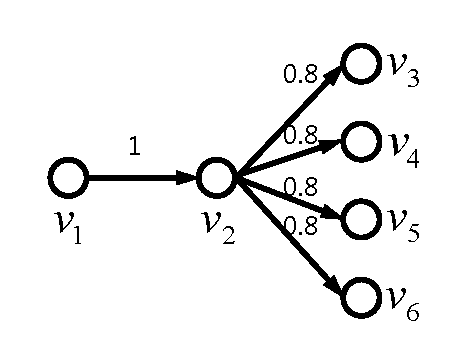
\includegraphics[width=0.8\linewidth]{figures/tinyGraph.pdf}
     \caption{社交网络中的信息传播概率图$\mathcal{G}$}\label{fig:tinyGraph}
   \end{minipage}
   \hfill
   \begin {minipage}{0.48\textwidth}
     \centering
     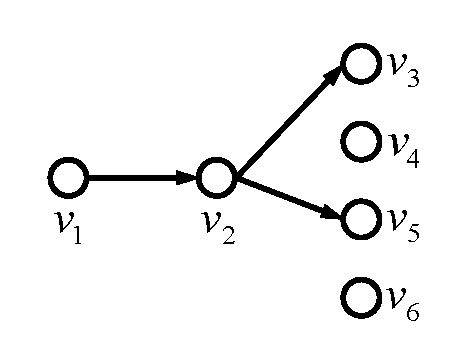
\includegraphics[width=0.8\linewidth]{figures/tinyRandomGraph.pdf}
     \caption{随机实例图$g$}\label{fig:tinyRandomGraph}
   \end{minipage}
\end{figure}

以图\ref{fig:tinyGraph}中的社交网络$\mathcal{G}$为例,考虑种子节点集合$S=\left\{v_1\right\}$的信息传播过程。图\ref{fig:tinyGraph}中边上的数值代表着节点之间的传播概率$p^\mathcal{G}_{u,v}$。整个信息传播的过程可以描述如下。在$t=0$时刻,由于节点$v_1$是种子节点集合中唯一的节点,因此节点$v_1$被激活。在$t=1$时刻,因为节点$v_1$在$t=0$时刻被激活,而且图$\mathcal{G}$中存在一条从$v_1$到$v_2$概率为1的边,节点$v_1$将依概率1去激活节点$v_2$。因此,节点$v_2$将在$t=1$时刻被激活,$S_1=\left\{v_2\right\}$。此后,在$t=2$时刻,节点$v_2$将尝试去激活节点$v_3$、$v_4$、$v_5$以及$v_6$。假设这一次信息传播过程如图\ref{fig:tinyRandomGraph}所示,节点$v_3$和$v_5$被激活,则$S_2=\left\{v_3, v_5\right\}$。然后,在$t=3$时刻,由于被激活的节点没有后继节点可被激活,整个信息传播过程在此时刻停止。定义$I\left(S\right)$为在种子节点集合是$S$的条件下,整个信息传播过程中激活的节点数目,代表信息传播过程中的影响力。在上述的图$\mathcal{G}$的一次信息传播过程中,影响力$I\left(S\right)=4$。

\subsection{传播效率最大化问题}
\label{3subsec:efficiency}

\section{方法描述}
\label{3sec:method}

\section{实验分析}
\label{3sec:experiment}

\section{本章小结}
\label{3sec:conclusion}

